\iffalse
\let\negmedspace\undefined
\let\negthickspace\undefined
\documentclass[journal,12pt,twocolumn]{IEEEtran}
\usepackage{cite}
\usepackage{amsmath,amssymb,amsfonts,amsthm}
\usepackage{algorithmic}
\usepackage{graphicx}
\usepackage{textcomp}
\usepackage{xcolor}
\usepackage{txfonts}
\usepackage{listings}
\usepackage{enumitem}
\usepackage{mathtools}
\usepackage{gensymb}
\usepackage{comment}
\usepackage[breaklinks=true]{hyperref}
\usepackage{tkz-euclide}
\usepackage{listings}
\usepackage{gvv}
\def\inputGnumericTable{}
\usepackage[latin1]{inputenc}
\usepackage{color}
\usepackage{array}
\usepackage{longtable}
\usepackage{calc}
\usepackage{multirow}
\usepackage{hhline}
\usepackage{ifthen}
\usepackage{lscape}

\newtheorem{theorem}{Theorem}[section]
\newtheorem{problem}{Problem}
\newtheorem{proposition}{Proposition}[section]
\newtheorem{lemma}{Lemma}[section]
\newtheorem{corollary}[theorem]{Corollary}
\newtheorem{example}{Example}[section]
\newtheorem{definition}[problem]{Definition}
\newcommand{\BEQA}{\begin{eqnarray}}
\newcommand{\EEQA}{\end{eqnarray}}
\newcommand{\define}{\stackrel{\triangle}{=}}
\theoremstyle{remark}
\newtheorem{rem}{Remark}
\begin{document}

\bibliographystyle{IEEEtran}
\vspace{3cm}

\title{NCERT Discrete - 11.9.2.6}
\author{EE23BTECH11212 - Manugunta Meghana Sai$^{*}$% <-this % stops a space
}
\maketitle
\newpage
\bigskip

\renewcommand{\thefigure}{\theenumi}
\renewcommand{\thetable}{\theenumi}

\vspace{3cm}
\textbf{NCERT Maths 11.9.2 Q6} 
If the sum of certain number of terms in a AP 25,22,19,... is 116. Find the last term.\\
\solution
\fi
\begin{table}[h!]
    \centering
    \begin{tabular}{|c|c|c|}
	\hline
	\textbf{Symbol} & \textbf{Value} & \textbf{Description} \\[6pt]
	\hline
	$x(0)$ & $25$ & first term of AP \\[6pt]
	\hline
	$d$ & $-3$ & common difference \\[6pt]
	\hline
	$x(n)$ & $(25-3n)u(n)$ & $n$-th term of AP \\[6pt]
	\hline
	$y(n)$ & $116$ & sum of terms \\[6pt]
	\hline 
\end{tabular}

    \caption{Input Parameters}
    \label{tab:table1}
\end{table}
\begin{align}
	x(n) = (25 - 3n)u(n)
	\label{eq:11.9.2.6}
\end{align}
Applying Z transform:
\begin{align}
    x(z) &=\frac{25}{1-z^{-1}} - \frac{3z^{-1}}{(1-z^{-1})^2}\\
    &= \frac{25-28z^{-1}}{(1-z^{-1})^2} 
\end{align}
     Region of Convergence or R.O.C :
\begin{align}
     \abs{z}>1
\end{align}
For AP, the sum of first n+1 terms can be written as :
\begin{align}
	 y(n)&=x(n)*u(n)
\end{align}  
Applying Z transform on both sides
\begin{align}
	Y(z) &= X(z)U(z)\\
	&=\frac{25}{(1-z^{-1})^2} - \frac{3z^{-1}}{(1-z^{-1})^3}
\end{align}
Using contour integration to find inverse Z transform:
\begin{align}
	y(n) &= \frac{1}{2\pi j} \oint_C Y(z) z^{n-1} dz\\
	&= \frac{1}{2\pi j} \oint_C \left[ \frac{25}{(1-z^{-1})^2} - \frac{3z^{-1}}{(1-z^{-1})^3} \right]z^{n-1} \, dz
\end{align}
The sum of the terms of the sequence is computed using the residue theorem, expressed as $R_i$, which represents the residue of the Z-transform at $ z=1 $ for the expression $ Y(z) $.
\begin{align}
	R_i=R_1 + R_2
\end{align}
 $R_1$ and $R_2$ are residues calculated at the poles of the Z-transform.
\begin{align}
		R_1 &= \frac{1}{{(2-1)!}} \left. \frac{d (25z^{n+1})}{dz} \right|_{z=1} \\
	&=25(n+1)
\end{align}
\begin{align}
	R_2 &= \frac{1}{{(3-1)!}} \left. \frac{d^2(-3z^{n+1})}{dz^2} \right|_{z=1} \\
	&= \frac{-3}{2}(n+1)(n)
\end{align}
The sum of terms is given by $R_i$:
 \begin{align}
25(n+1)	+ \frac{-3}{2} n(n+1) = 116 
 \end{align}
Solving the equation gives :
\begin{align}
	n&=7\\ n&=8.667
\end{align}
Since n can take only integer values, $n=8.667$ is rejected. 
Upon substituting the value of n in equation~\eqref{eq:11.9.2.6}:
\begin{align}
	x(7)=4
\end{align}
Hence the last term of the given AP is 4.
\begin{figure}[h!]
    \centering
    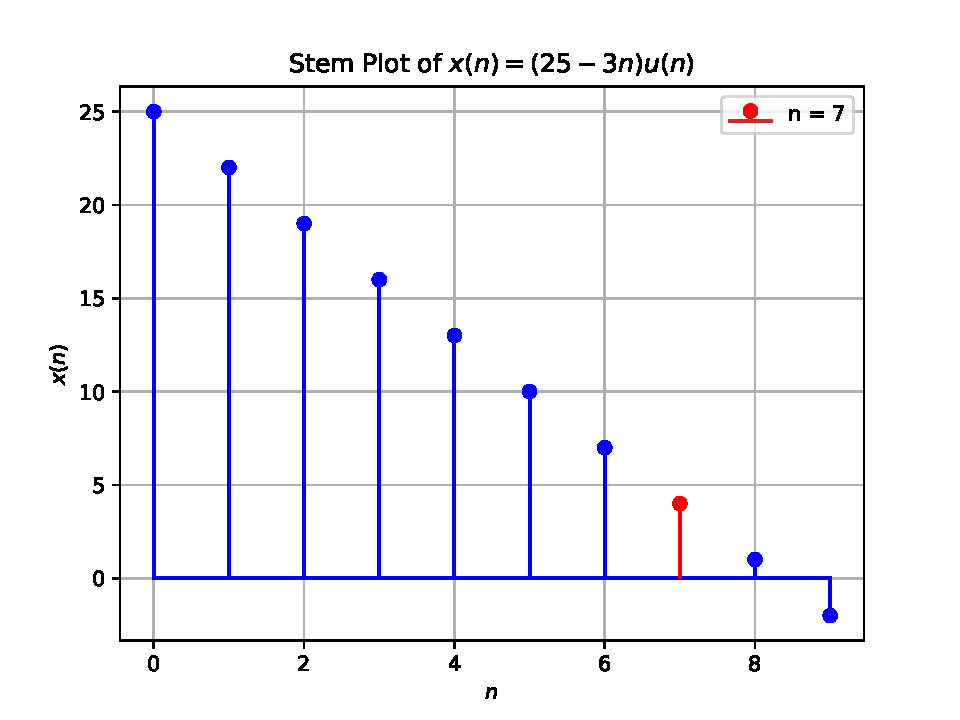
\includegraphics[width=\columnwidth]{ncert-maths/11/9/2/6/figs/stem_plot.pdf}
\end{figure}
%\end{document}
